%
% HSR LaTex Template
% Copyright 2012, Florian Bentele / modified 2015 - Martin Stypinski
%
% Complete LaTex template for thesis at HSR, customized
% for Prof. Dr. Peter Heinzmann
%
%
% This document is free software: you can redistribute
% it and/or modify it under the terms of the GNU
% General Public License as published by the Free
% Software Foundation, either version 3 of the License,
% or (at your option) any later version.
%
% This document is distributed in the hope that it will
% be useful, but WITHOUT ANY WARRANTY; without even the
% implied warranty of MERCHANTABILITY or FITNESS FOR A
% PARTICULAR PURPOSE. See the GNU General Public
% License for more details.
%
% You should have received a copy of the GNU General
% Public License along with this document. If not, see
% <http://www.gnu.org/licenses/>.
%

\newcommand{\styp}{Martin Stypinski}

\documentclass[11pt]{hsrthesis}

% The following snippet is copied from this stack overflow answer
% http://stackoverflow.com/a/3175141
% It sets the color right for lstlisting, so that we 
% can include code snippet
\definecolor{dkgreen}{rgb}{0,0.6,0}
\definecolor{gray}{rgb}{0.5,0.5,0.5}
\definecolor{mauve}{rgb}{0.58,0,0.82}

\lstset{frame=tb,
	language=Java,
	aboveskip=3mm,
	belowskip=3mm,
	showstringspaces=false,
	columns=flexible,
	basicstyle={\small\ttfamily},
	numbers=none,
	numberstyle=\tiny\color{gray},
	keywordstyle=\color{blue},
	commentstyle=\color{dkgreen},
	stringstyle=\color{mauve},
	breaklines=true,
	breakatwhitespace=true,
	tabsize=3
}

\makeindex

\makeglossaries

\newglossaryentry{RDBMS}{
	name=RDBMS,
	description={Find better defintion },
	first={Relational Database Management Systems (RDBMS)}
}

\newglossaryentry{DSMS}{
	name=DSMS,
	description={Data stream managment systems are database systems to handle continuous streams of data.},
	first={Data Stream Management Systems (DSMS)}
}


\begin{document}
\newcommand{\thesistitle}{Data Stream Management Systems: \\ \textbf{Apache Spark Streaming}}
\newcommand{\thesissubtitle}{Seminar: “Advanced Database Systems”}
\newcommand{\thesisauthora}{Martin Stypinski}
\newcommand{\thesisauthorb}{}
\newcommand{\thesisauthorc}{}
\newcommand{\professor}{Prof. Stefan F. Keller}
\newcommand{\departement}{Master of Science in Engineering}
\newcommand{\school}{Hochschule für Technik Rapperswil}
\newcommand{\term}{Herbstsemester 2016/2017}
\newcommand{\thedate}{\today}
\newcommand{\timeperiode}{19.09.2016 - 23.12.2015}
\newcommand{\workload}{90 Stunden, 3 ECTS}
\newcommand{\linktothesis}{https://github.com/Styp/HSR_DBSeminar}

\maketitle


\newpage

\pagenumbering{roman}

\newpage

% The main content
%%%%%%%%%%%%%%%%%%
\newpage
\cleardoublepage
\phantomsection
\addcontentsline{toc}{chapter}{Abstract}
\chapter*{Abstract}

This will be the abstract - eventually ;)


% Table of content
% % % % % % % % %
\newpage
\addcontentsline{toc}{chapter}{Inhaltsverzeichnis}
\tableofcontents
\newpage

\pagenumbering{arabic}
\setcounter{page}{1}

\chapter{Introduction}

This paper is the result of the seminar on "Advanced Database Systems" at the University of Applied Science Rapperswil. The paper shall cover all the necessary concepts of "Streaming Database Systems" and investigating one particular product for its abilities. The product is determined to be "Apache Spark Streaming" which is well known to be used in companies handling big data flows for daily business like Uber\cite{uber}, Netflix and Pinterest.

\section{Motivation}
Modern \Gls{RDBMS} show the perfect snapshot of the past, while modern businesses rely heavily on data, these concepts become limiting. While there is a need for storage and persistence, where \Gls{RDBMS}s are still in their prime, there is another need for real time data processing. Real time data processing can be useful to give an accurate anticipation about the future. This use case is a driving force to justify an new database concept for data streams - the \Gls{DSMS} is born. 
\\
\subsection{Fundamentals of database systems}
To gain further insights and justify the need for new concepts, it is necessary to have a look at already given and proven concepts. Fundamentals of database systems require to understand the concept of the CAP-Theorem. The CAP-Theorem was first introduced by Eric Brewer in 2000 and later verified.
\\
\blockquote{When designing distributed web services, there are three properties that are commonly desired: consistency, availability, and partition tolerance. It is impossible to achieve all three.} \cite[S. 1]{Gilbert:2002:BCF:564585.564601}

\begin{figure}[H]
	\centering
%	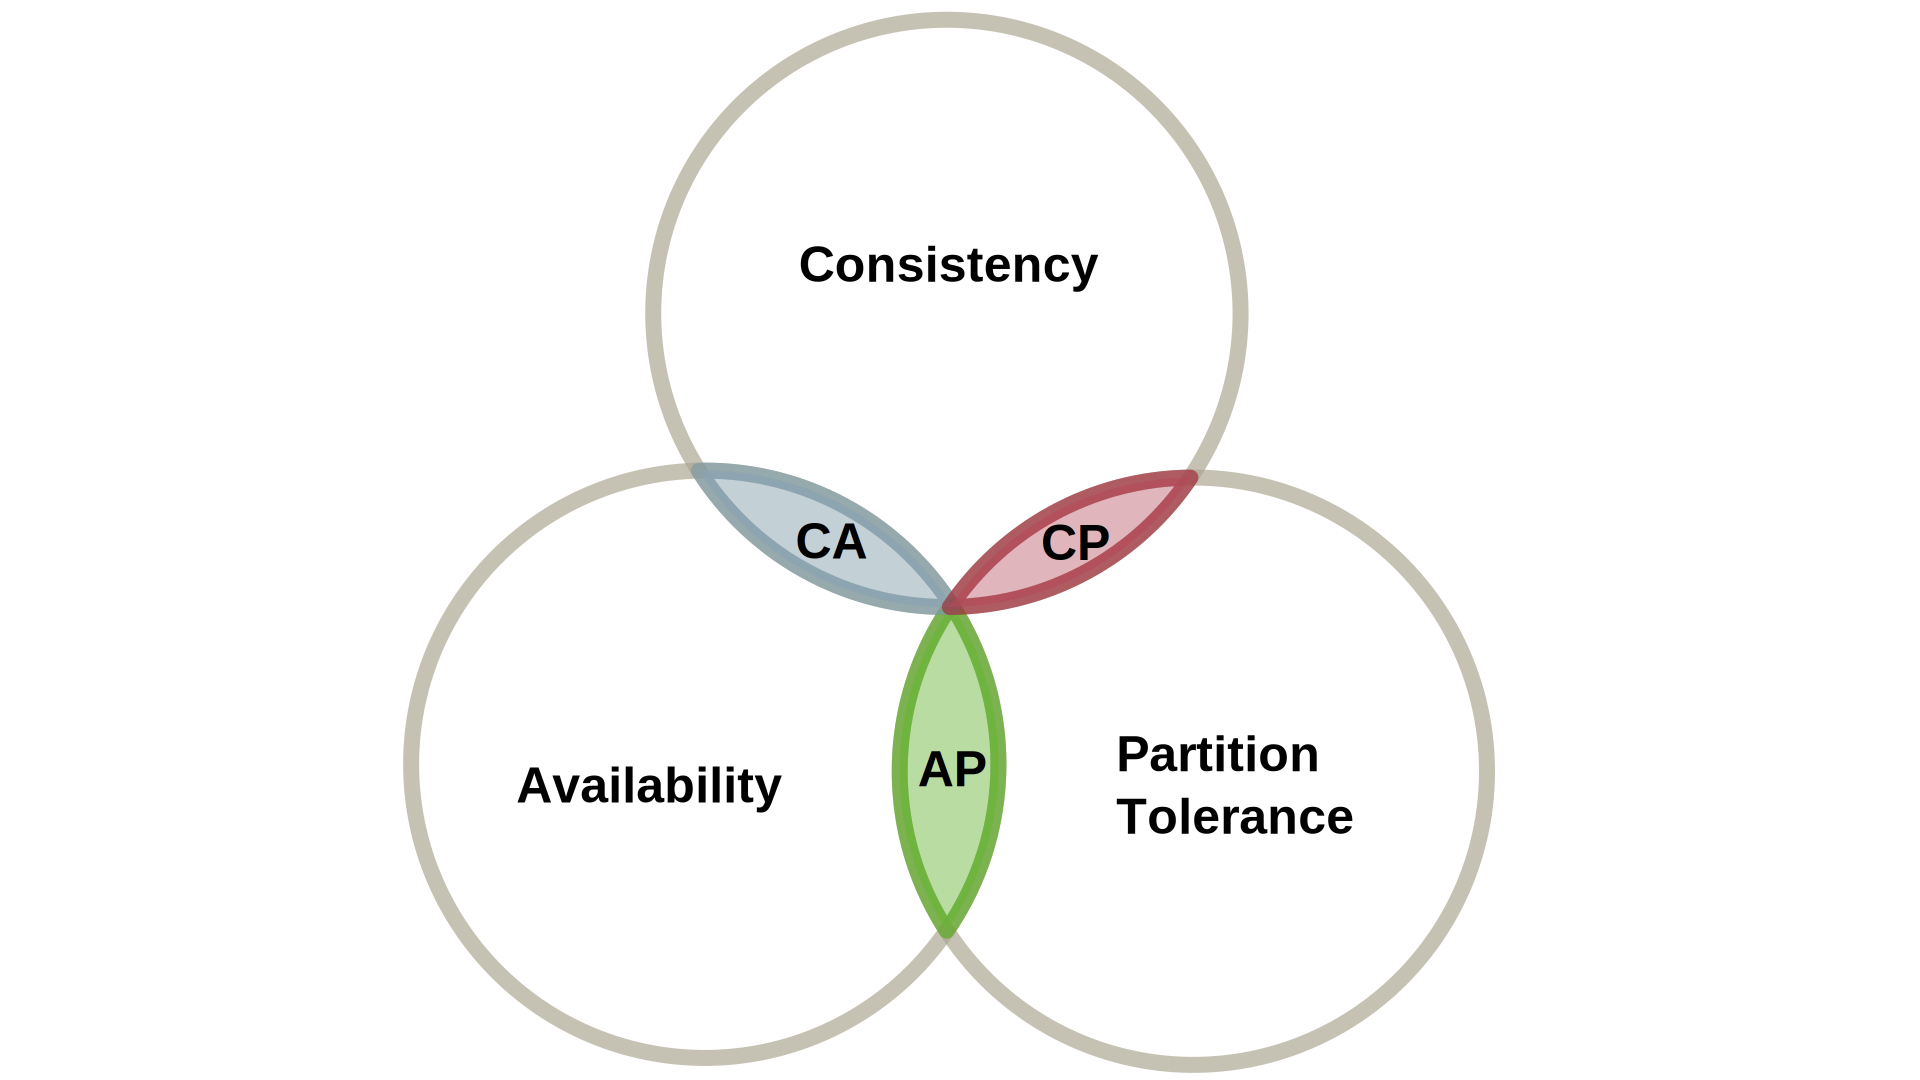
\includegraphics[width=0.8\textwidth]{images/cap.pdf}
	\caption{Übersicht der Project Helin Architektur }
	\label{fig:architecture-overview}
\end{figure}


\begin{itemize}
	\item{\textbf{Consistency:} Guarantees that a read will receive the most recent data or an error.}
	\item{\textbf{Availability:} Every request will get a response, although no guarantee on correctness of the data. }
	\item{\textbf{Partition Tolerance:} The system can operate although parts of it are unavailable due to network or hardware failure.}
	
\end{itemize}

Furter figure (xyz) illustrates this with three circles and indicates that the intersection of two of them enables further technology. These areas are important for todays database technology.


\begin{itemize}
	\item{\textbf{CA} Consistency \& Availability: \\
	All RDBMS that follow the ACID theorem can be found here. Consistency is uf utmost importance. (\textit{PostgreSQL})}
	\item{\textbf{AP} Availability \& Partition Tolerance: \\
	Most NoSQL technology can be found here and systems that follow the BASE theorem. The consistency is 'relaxed' but the availability and distributed performance can therefore be imporved! }
	\item{\textbf{PC} Consistency \& Partition Tolerance: \\
	Acid based distributed databases can be found here, often a 'read-any' and 'write all' scheme is implemented.}
\end{itemize}

All these systems lead to a common subset of operations. All data objects can be created, read, updated and deleted (CRUD). This implies the database to act as a central storage, but what if data is time critical or due to internet trafic not consitence. The importance of the storage shifts towards a central subscription system.

But what happens, if time critical applications need to evaluate data and the 
\begin{figure}[H]
	\centering
	\includegraphics[scale=1]{images/DBMS_overview.png}
	\caption{Übersicht der Project Helin Architektur }
	\label{fig:architecture-overview}
\end{figure}

\begin{tabular}{lll}


\end{tabular}



\begin{figure}[H]
	\centering
	\includegraphics[width=1\textwidth]{images/DSMS_overview.png}
	\caption{Übersicht der Project Helin Architektur }
	\label{fig:architecture-overview}
\end{figure}



% The main content
%%%%%%%%%%%%%%%%%%




% Templates
%%%%%%%%%%%%%%%%%%%%%%%%%%%%
%\newpage
%\input{chapter/99_demo/demo}

% List of figures & glossary
%%%%%%%%%%%%%%%%%%%%%%%%%%%%

\listoffigures

\clearpage

\printglossary[style=altlist,title=Glossar]

% Bibliography
%%%%%%%%%%%%%%
\bibliographystyle {alpha}
\bibliography{index/bibliography}



\end{document}